%
% ---------------------------------------------------------------
% Copyright (C) 2012-2018 Gang Li
% ---------------------------------------------------------------
%
% This work is the default powerdot-tuliplab style test file and may be
% distributed and/or modified under the conditions of the LaTeX Project Public
% License, either version 1.3 of this license or (at your option) any later
% version. The latest version of this license is in
% http://www.latex-project.org/lppl.txt and version 1.3 or later is part of all
% distributions of LaTeX version 2003/12/01 or later.
%
% This work has the LPPL maintenance status "maintained".
%
% This Current Maintainer of this work is Gang Li.
%
%

\documentclass[
size=14pt,
paper=smartboard,  %a4paper, smartboard, screen
mode=present, 		%present, handout, print
display=slides, 	% slidesnotes, notes, slides
style=tuliplab,  	% TULIP Lab style
pauseslide,
fleqn,leqno]{powerdot}

\usepackage{cancel}
\usepackage{caption}
\usepackage{stackengine}
\usepackage{smartdiagram}
\usepackage{attrib}
\usepackage{amssymb}
\usepackage{amsmath} 
\usepackage{amsthm} 
\usepackage{mathtools}
\usepackage{rotating}
\usepackage{graphicx}
\usepackage{boxedminipage}
\usepackage{rotate}
\usepackage{calc}
\usepackage[absolute]{textpos}
\usepackage{psfrag,overpic}
\usepackage{fouriernc}
\usepackage{pstricks,pst-3d,pst-grad,pstricks-add,pst-text,pst-node,pst-tree}
\usepackage{moreverb,epsfig,subfigure}
\usepackage{color}
\usepackage{booktabs}
\usepackage{etex}
\usepackage{breqn}
\usepackage{multirow}
\usepackage{natbib}
\usepackage{bibentry}
\usepackage{gitinfo2}
\usepackage{siunitx}
\usepackage{nicefrac}
%\usepackage{geometry}
%\geometry{verbose,letterpaper}
\usepackage{media9}
\usepackage{animate}
%\usepackage{movie15}
\usepackage{auto-pst-pdf}
\usepackage{breakurl}
\usepackage{fontawesome}
\usepackage{xcolor}
\usepackage{multicol}
\usepackage{verbatim}
\usepackage[utf8]{inputenc}
\usepackage{dtk-logos}
\usepackage{tikz}
\usepackage{adigraph}
%\usepackage{tkz-graph}
\usepackage{hyperref}
%\usepackage{ulem}
\usepackage{pgfplots}
\usepackage{verbatim}
\usepackage{fontawesome}
\usepackage{todonotes}
% \usepackage{pst-rel-points}
\usepackage{animate}
\usepackage{fontawesome}
\usepackage{listings}
\lstset{frameround=fttt,
	frame=trBL,
	stringstyle=\ttfamily,
	backgroundcolor=\color{yellow!20},
	basicstyle=\footnotesize\ttfamily}
\lstnewenvironment{code}{
	\lstset{frame=single,escapeinside=`',
		backgroundcolor=\color{yellow!20},
		basicstyle=\footnotesize\ttfamily}
}{}


%\usepackage{hyperref}
\hypersetup{ % TODO: PDF meta Data
	pdftitle={Presentation Title},
	pdfauthor={Gang Li},
	pdfpagemode={FullScreen},
	pdfborder={0 0 0}
}


% \usepackage{auto-pst-pdf}
% package to show source code

\definecolor{LightGray}{rgb}{0.9,0.9,0.9}
\newlength{\pixel}\setlength\pixel{0.000714285714\slidewidth}
\setlength{\TPHorizModule}{\slidewidth}
\setlength{\TPVertModule}{\slideheight}
\newcommand\highlight[1]{\fbox{#1}}
\newcommand\icite[1]{{\footnotesize [#1]}}

\newcommand\twotonebox[2]{\fcolorbox{pdcolor2}{pdcolor2}
	{#1\vphantom{#2}}\fcolorbox{pdcolor2}{white}{#2\vphantom{#1}}}
\newcommand\twotoneboxo[2]{\fcolorbox{pdcolor2}{pdcolor2}
	{#1}\fcolorbox{pdcolor2}{white}{#2}}
\newcommand\vpspace[1]{\vphantom{\vspace{#1}}}
\newcommand\hpspace[1]{\hphantom{\hspace{#1}}}
\newcommand\COMMENT[1]{}

\newcommand\placepos[3]{\hbox to\z@{\kern#1
		\raisebox{-#2}[\z@][\z@]{#3}\hss}\ignorespaces}

\renewcommand{\baselinestretch}{1.2}


\newcommand{\draftnote}[3]{
	\todo[author=#2,color=#1!30,size=\footnotesize]{\textsf{#3}}	}
% TODO: add yourself here:
%
\newcommand{\gangli}[1]{\draftnote{blue}{GLi:}{#1}}
\newcommand{\shaoni}[1]{\draftnote{green}{sn:}{#1}}
\newcommand{\gliMarker}
{\todo[author=GLi,size=\tiny,inline,color=blue!40]
	{Gang Li has worked up to here.}}
\newcommand{\snMarker}
{\todo[author=Sn,size=\tiny,inline,color=green!40]
	{Shaoni has worked up to here.}}

%%%%%%%%%%%%%%%%%%%%%%%%%%%%%%%%%%%%%%%%%%%%%%%%%%%%%%%%%%%%%%%%%%%%%%%%
% title
% TODO: Customize to your Own Title, Name, Address
%
\title{HOUSE PRICES-ADVANCED REGRESSION TECHNIQUES}
\author{
	Tao Wang
	\\
	\\University of Chinese Academy of Sciences
}
\date{\gitCommitterDate}


% Customize the setting of slides
\pdsetup{
	% TODO: Customize the left footer, and right footer
	rf=\href{http://www.tulip.org.au}{
		Last Changed by: \textsc{\gitCommitterName}\- (\gitAuthorDate)
	},
	cf={HOUSE PRICES-ADVANCED REGRESSION TECHNIQUES},
}

\begin{document}
	\maketitle
	\begin{slide}[toc=,bm=]{Overview}
		\tableofcontents[content=currentsection,type=1]
	\end{slide}

	\section{Project Description \& Evaluation}
	\begin{slide}[toc=,bm=]{Project Description \& Evaluation}
	\begin{center}
		\twotonebox{\rotatebox{90}{Descripion}}{\parbox{.86\textwidth}
			{For home buyers, they generally do not buy homes with basements or near railroads, and there are other features of a home that can even much more influence the price of a home than the number of bedrooms. \\ This project provides 79 characteristics of a house that are used to predict the price of a house.\\}
			}
	\end{center}
	\begin{center}
		\twotonebox{\rotatebox{90}{Evaluation}}{\parbox{.86\textwidth}
			{There are 1459 data in the test set, and the output contains ID numbers and predicted house prices. Submissions are evaluated on Root-Mean-Squared-Error(RMSE) between the logarithm of the predicted value and the logarithm of the observed sales price.\\}
			}
	\end{center}
	\end{slide}

	\section{Dataset Description}
	\begin{slide}[toc=,bm=]{File Description}
	\begin{itemize}
		\item train.csv - the training set
		\item test.csv - the test set
		\item data˙description.txt - full description of each column, originally prepared by	Dean De Cock but lightly edited to match the column names used here
		\item sample˙submission.csv - a benchmark submission from a linear regression on year and month of sale, lot square footage, and number of bedrooms
	\end{itemize}
	\end{slide}
	\begin{slide}[toc=,bm=]{Outlying Aspects Mining vs Outlier Detection}
		There are 79 variables of inconsistent types, some discrete and some continuous, and after data processing, the variables of type object can be seen as follows:\\
		\begin{center}
			\begin{tabular}{c c c c}
				\toprule
				%\centering
				\# & \texttt{Column}  & \texttt{Non-Null Count} & \texttt{Dtype} \\
				\midrule
				$0$
				&  {$MSZoning$} &  {$1460 non-null$} &  {$object$}  \\
				$1$
				&  {$Street$} &  {$1460 non-null$}&  {$object$} \\
				$2$
				&  {$Alley$} &  {$91 non-null$} &  {$object$} \\
				$3$
				&  {$LotShape$} &  {$1460 non-null$}&  {$object$} \\
				$...$
				&  {$...$} &  {$...$} &  {$object$}\\
				\bottomrule
			\end{tabular}
		\end{center}
		The characteristics of variables of type object are represented by string,such as:
		\begin{center}
			\begin{tabular}{c c}
				\toprule
				%\centering
				\multicolumn{2}{c}{Mszoning:Identifies the general zoning classfication of the sale} \\ 
				\midrule
				$A$ &  {$Agriculture$}  \\
				$C$ &  {$Commercial$}  \\
				$...$ &  {$...$}  \\
				\bottomrule
			\end{tabular}
		\end{center}	
	\end{slide}
	\begin{slide}[toc=,bm=]{Outlying Aspects Mining vs Outlier Detection}
		The numeric variables are as follows:
		\begin{center}
			\begin{tabular}{c c c c}
				\toprule
				%\centering
				\# & \texttt{Column}  & \texttt{Non-Null Count} & \texttt{Dtype} \\
				\midrule
				$0$
				&  {$MSZoning$} &  {$1460 non-null$} &  {$int64$}  \\
				$1$
				&  {$Street$} &  {$1460 non-null$}&  {$int64$} \\
				$2$
				&  {$Alley$} &  {$1201 non-null$} &  {$float64$} \\
				$3$
				&  {$LotShape$} &  {$1460 non-null$}&  {$int64$} \\
				$...$
				&  {$...$} &  {$...$} &  {$...$}\\
				\bottomrule
			\end{tabular}
		\end{center}
	\end{slide}
	\section{Data Pre-processing}
	\begin{slide}[toc=,bm=]{Date Pre-Processing}
		\begin{itemize}
		\item Number of missing data in the training set:
		\begin{center}
			\begin{tabular}{c c c }
				\toprule
				%\centering
				$type$ & \texttt{num}  & \texttt{persent} \\
				\midrule
				$PoolQC$ &  {$1453$} &  {$0.995$}   \\
				$MiscFecture$ &  {$1406$} &  {$0.963$}   \\
				$Alley$ &  {$1369$} &  {$0.938$}   \\
				$Fence$ &  {$1179$} &  {$0.808$}   \\
				$FireplaceQu$ &  {$690$} &  {$0.472$}   \\
				$LotFronttage$ &  {$259$} &  {$0.177$}   \\
				$GarageType$ &  {$81$} &  {$0.055$}   \\
				$GarageYrBlt$ &  {$81$} &  {$0.555$}   \\
				$GarageFinish$ &  {$81$} &  {$0.555$}   \\
				 {$...$} &  {$...$}  &  {$...$}\\
				\bottomrule
			\end{tabular}
		\end{center}
		\end{itemize}
	\end{slide}
	\begin{slide}[toc=,bm=]{Date Pre-Processing}
		\begin{itemize}
			\item Number of missing data in the test set:
			\begin{center}
				\begin{tabular}{c c c }
					\toprule
					%\centering
					$type$ & \texttt{num}  & \texttt{persent} \\
					\midrule
					$PoolQC$ &  {$1456$} &  {$0.997$}   \\
					$MiscFecture$ &  {$1408$} &  {$0.964$}   \\
					$Alley$ &  {$1352$} &  {$0.926$}   \\
					$Fence$ &  {$1169$} &  {$0.800$}   \\
					$FireplaceQu$ &  {$730$} &  {$0.5$}   \\
					$LotFronttage$ &  {$227$} &  {$0.155$}   \\
					$GarageYrBlt$ &  {$78$} &  {$0.053$}   \\
					$GarageFinish$ &  {$78$} &  {$0.053$}   \\
					{$...$} &  {$...$}  &  {$...$}\\
					\bottomrule
				\end{tabular}
			\end{center}
		\end{itemize}
	\end{slide}
	\begin{slide}[toc=,bm=]{Data cleaning of training set}
		\begin{center}
			\twotonebox{\rotatebox{90}{Step1}}{\parbox{.86\textwidth}
				{We choose to remove the feature PoolQC, MiscFeature, Alley,Fence and FireplaceQu because we do not have a suitable method to replenish a large amount of data.\\}
			}
		\end{center}
		\begin{center}
			\twotonebox{\rotatebox{90}{Step2}}{\parbox{.86\textwidth}
				{Since the propeties of numeric types are conveniently complemented by medians or averages, etc. We first examine the properties of numeric types.\\
				We first examine the properties of numeric types. After studying it, we can find that only LotFrontage, MasVnrArea and GarageYrlBlt have missing features for the number types in the training set.\\
				For the masvnrarea with only 8 missing numbers, we can use the average to fill in, while for the other two with more missing numbers, we choose to use the plural to fill in.}
			}
		\end{center}
	\end{slide}
	\begin{slide}[toc=,bm=]{Data cleaning of training set}
		\begin{center}
			\twotonebox{\rotatebox{90}{Step3}}{\parbox{.86\textwidth}
				{ For some positively biased data, we try to use log transformation to reduce their skewness. By using function displot, we can find that the
				feature LotArea have positive skew like figure1.\\}
			}
		\end{center}
		\begin{figure}
			\centering
			\selectcolormodel{rgb}
			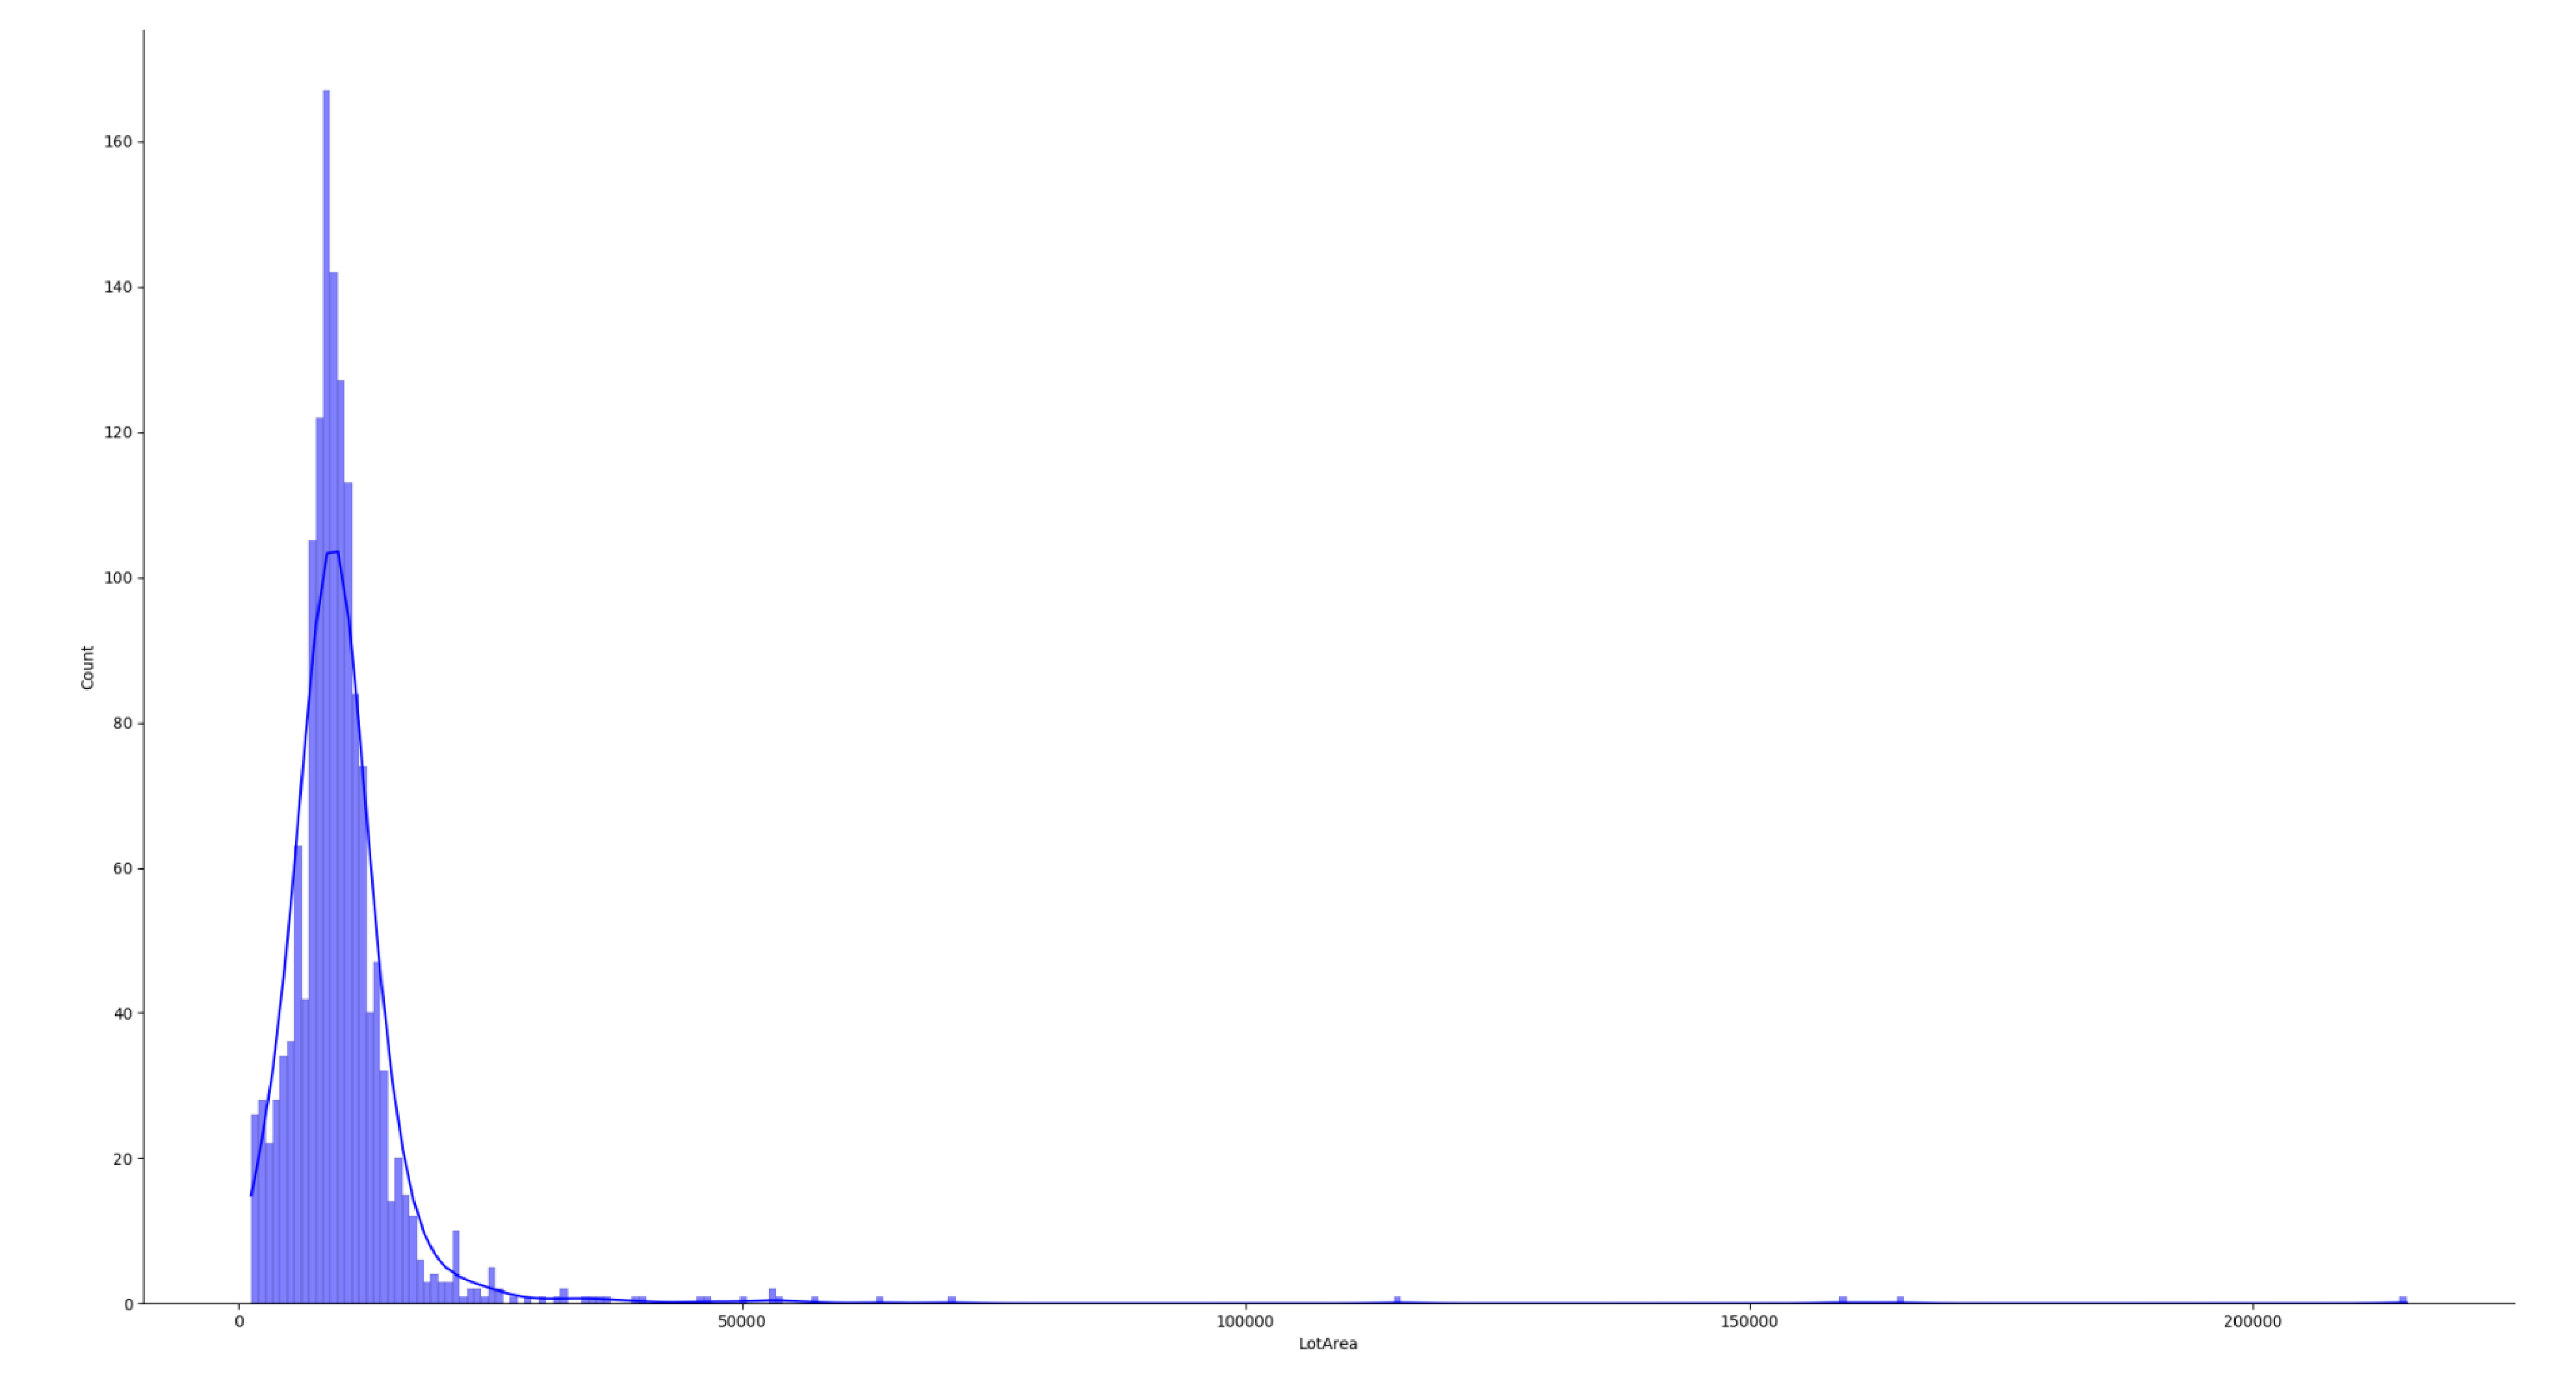
\includegraphics[width=0.6\textwidth]{../Data/Fig6.eps}\\
			\caption{An example of positive skew}
		\end{figure}
	\end{slide}
	\begin{slide}[toc=,bm=]{Data cleaning of training set}
		\begin{center}
			\twotonebox{\rotatebox{90}{Step4}}{\parbox{.86\textwidth}
				{Some of the data will be unreasonable, may be too large or too small. We need to remove this data before we put it into the training model.
				We first use the data visualization to look at it and decide on the removal
				method in figure2.\\}
			}
		\end{center}
		\begin{figure}
			\centering
			\selectcolormodel{rgb}
			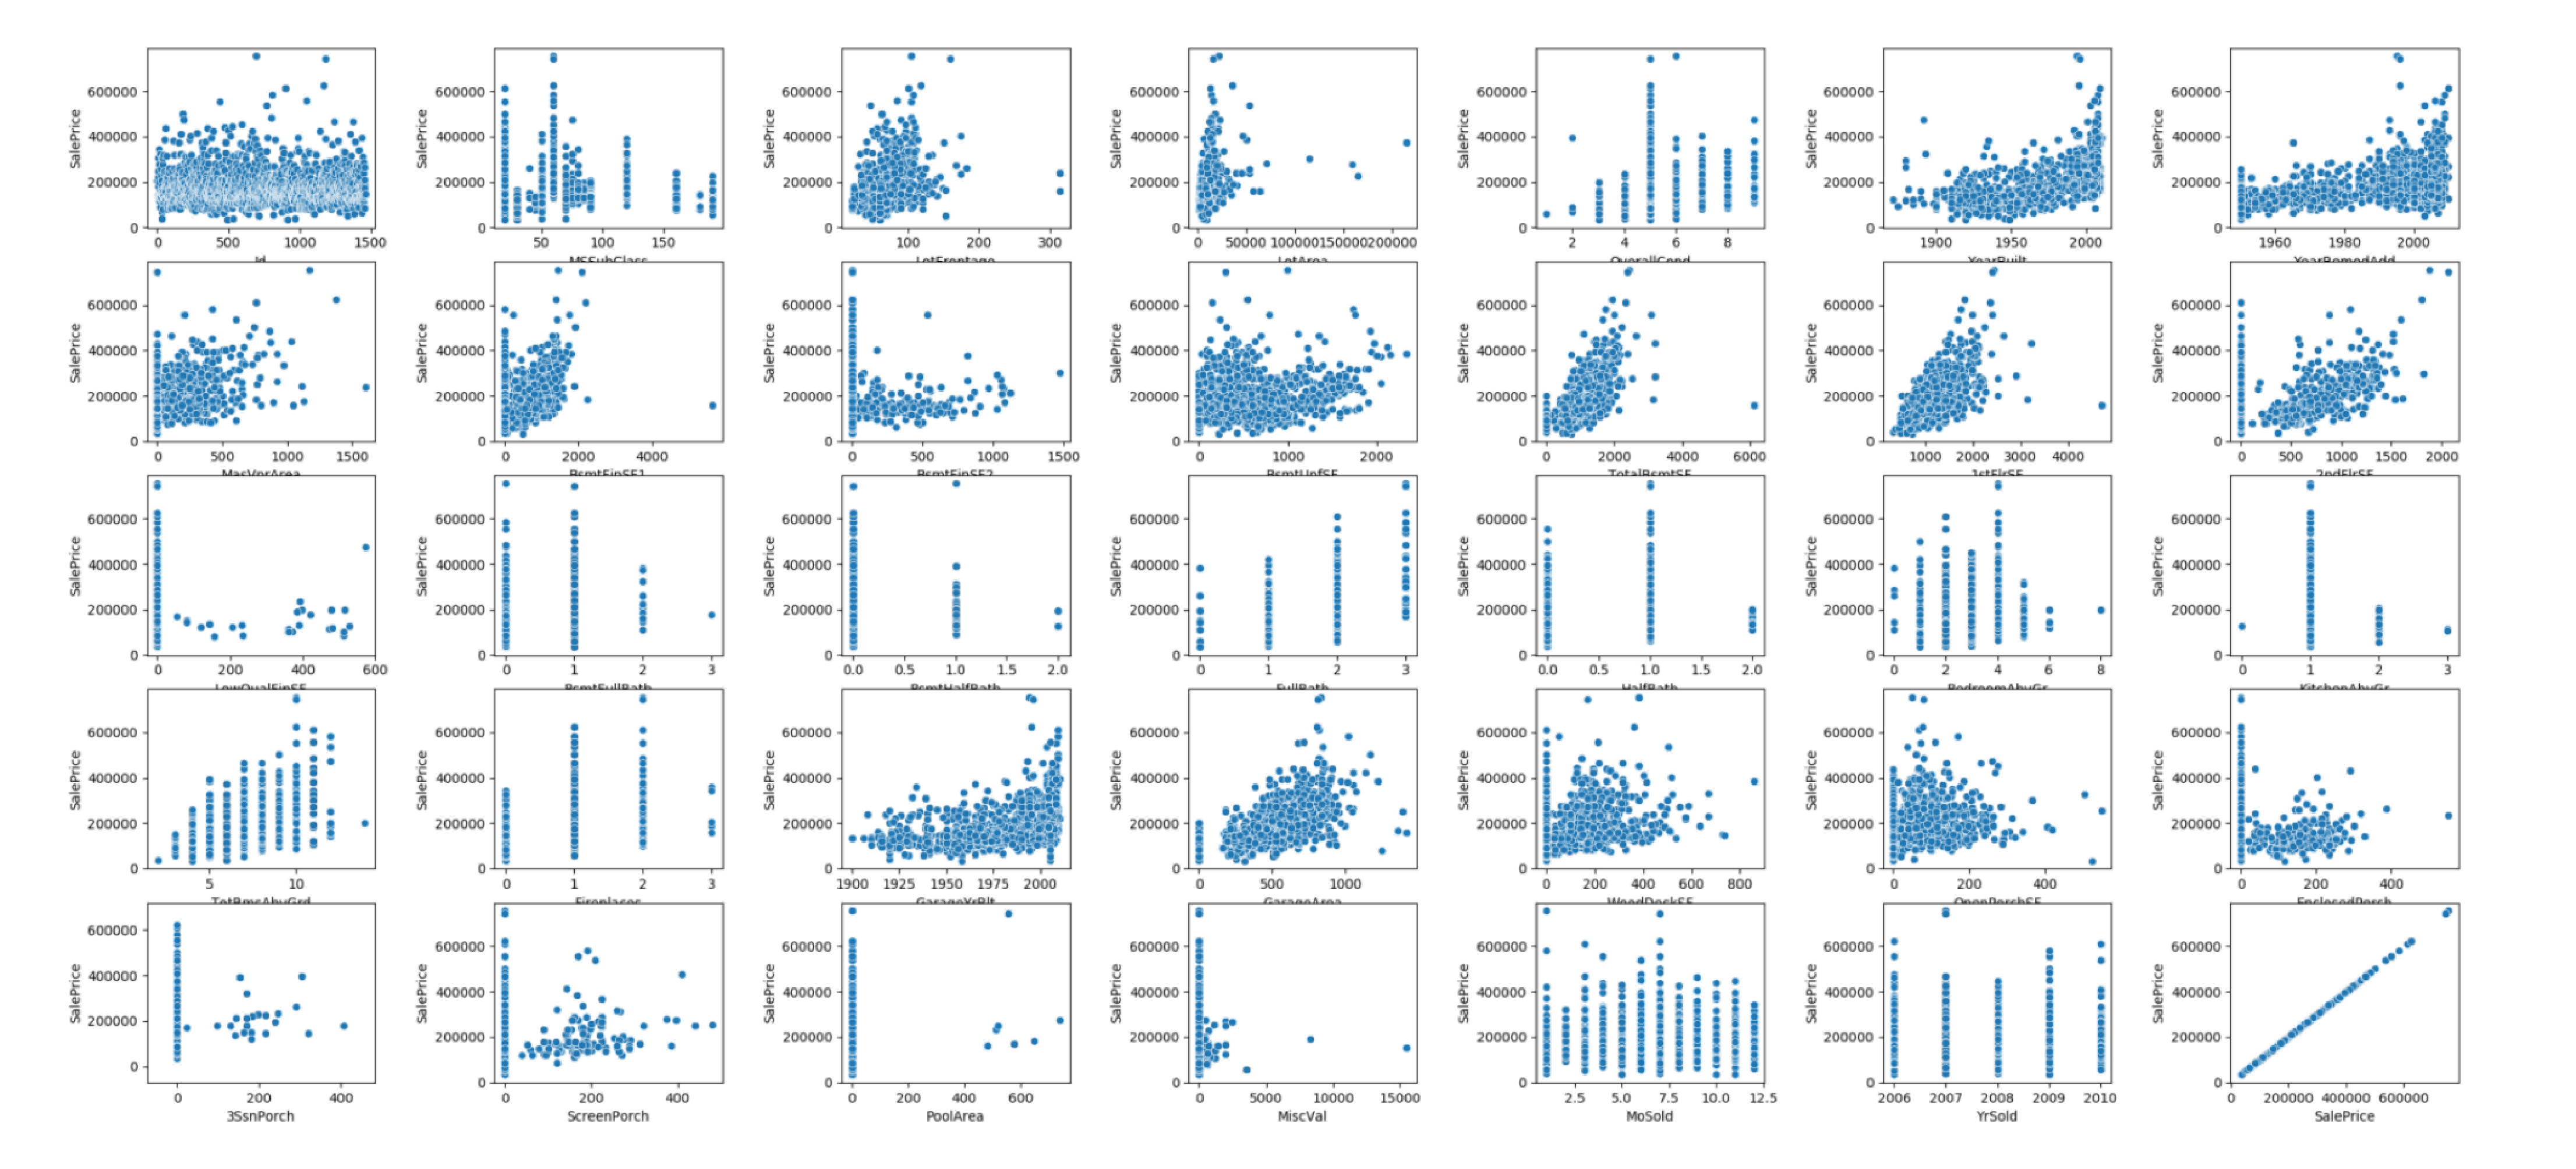
\includegraphics[width=0.7\textwidth]{../Data/Fig7.eps}\\
			\caption{Visualization of Training data}
		\end{figure}
	\end{slide}

	\begin{slide}[toc=,bm=]{Data cleaning of training set}
		\begin{center}
			\twotonebox{\rotatebox{90}{Step5}}{\parbox{.86\textwidth}
				{Now, we analyze the categorical data. For this string type of data, we choose to use the plural to fill in the missing data.}
			}
		\end{center}
		\begin{itemize}
			\item Data cleaning of testing set
			 All the previous steps are the same, but with the previous steps, we can find that the missing data in the test set is not the same as the training set, so we just need to simultaneously use the same analysis idea for these new missing data.\\
			 \item Date normalization and removal of weakly correlated data
			 After we clean the training and test set data, we need to consider if all the characteristics are related to the sales price. So we calculate the correlation coefficient of each characteristic and the sales price, we consider the correlation coefficient below 0.3 as almost irrelevant and remove these characteristics
		\end{itemize}
	\end{slide}
	\section{Training Result}
	\begin{slide}[toc=,bm=]{Training Result Summary}
			\begin{center}
				\begin{tabular}{c c }
					\toprule
					%\centering
					$method$ & \texttt{result}  \\
					\midrule
					$Linear Regression (low_corr deleted)$ &  {$0.7313$}   \\
					$Random Forest(low_corr deleted)$ &  {$0.16099$}   \\
					$K-neighbor(low_corr deleted)$ &  {$0.22111$}   \\
					$Adaboost Regressor(low_corr deleted)$ &  {$0.22124$}    \\
					$Xgboost(low_corr deleted)$ &  {$0.0.60098$}    \\
					$Xgboost$ &  {$0.17429$}    \\
					$Gradient Boosting Regressor(low_corr deleted)$ &  {$0.15922$}    \\
					$Gradient Boosting Regressor$ &  {$0.14173$}     \\
					\bottomrule
				\end{tabular}
			\end{center}
	\end{slide}
	\section{Conclusion}
\end{document}